\documentclass[11pt]{article}

\usepackage{thumbpdf, amssymb, amsmath, amsthm, microtype, array,
graphicx, verbatim, listings, color, fancybox}
\usepackage[pdftex]{hyperref}
\usepackage{mathtools}
\usepackage{graphicx}
\usepackage{caption}
\usepackage{setspace}
\usepackage{hyperref}
\usepackage{booktabs}
\usepackage{boxedminipage}
\usepackage{mathtools}
\usepackage[linesnumbered,ruled]{algorithm2e}
\usepackage{subcaption}
\usepackage{hyperref}
\usepackage{graphicx}
\usepackage{caption}
\usepackage{subcaption}
\usepackage{thmtools}
\usepackage{bbm}
\usepackage{pgf,tikz}
\usepackage{mathrsfs}
\usetikzlibrary{arrows}
\pagestyle{plain}
\usepackage[margin=1.2in]{geometry}
%\usepackage{arlhw}
\usepackage{multicol,multirow}
\usepackage{tikz}


\usepackage{thmtools}
\usepackage{thm-restate}

\usepackage{hyperref}

\usepackage{cleveref}

\declaretheorem[name=Theorem,numberwithin=section]{thm}
\newcommand{\oc}{\mathrm{oc}}
\newcommand{\mcc}{\mathcal{C}}
\newcommand{\NP}{\mathrm{NP}}
\newcommand{\Pp}{\mathrm{P}}
\newcommand{\UGC}{\mathrm{UGC}}
\newcommand{\W}{\mathrm{W}}
\newcommand{\FPT}{\mathrm{FPT}}
\newcommand{\opt}{\mathrm{OPT}}
\newcommand\floor[1]{\lfloor#1\rfloor}
\newcommand\ceil[1]{\lceil#1\rceil}
\newcommand{\FF}{\mathbb{F}}
\newcommand{\AF}{\mathbb{A}}
\newcommand{\BF}{\mathbb{A}}
\newcommand{\CF}{\mathbb{C}}

\newcommand{\subtour}{{\textsc{Subtour}}}

\newcommand{\Ex}{\mathop{\mathbb{E}}}


\usepackage{amsmath}
\theoremstyle{plain}
\newtheorem{theorem}{Theorem}
\newtheorem{corollary}{Corollary}[theorem]
\newtheorem*{main}{Main Theorem}
\newtheorem{lemma}{Lemma}
\newtheorem{question}{Question}
\newtheorem{conjecture}{Conjecture}
\newtheorem{fact}{Fact}
\newtheorem{observation}{Observation}
\newtheorem{proposition}{Proposition}
\theoremstyle{definition}
\newtheorem{define}{Definition}
\theoremstyle{claim}
\newtheorem{claim}{Claim}
\theoremstyle{remark}
\newtheorem*{notation}{Notation}
\theoremstyle{remark}
\newtheorem*{remark}{Remark}
\theoremstyle{remark}
\newtheorem{example}{\textbf{Example}}%[section]
\DeclareMathOperator{\chord}{chord}
\DeclareMathOperator{\ccover}{CYCLE-COVER}
\DeclareMathOperator{\degree}{deg}
\DeclareMathOperator{\connector}{CONNECTOR}
\DeclareMathOperator{\join}{JOIN}
\DeclareMathOperator{\cut}{CUT}
\DeclareMathOperator{\oddcut}{ODD-CUT}
\DeclareMathOperator{\cover}{COVER}
\DeclareMathOperator{\lp}{LP}
\DeclareMathOperator{\statecut}{STATE-CUT}
\DeclareMathOperator{\LPC}{Branching}
\DeclareMathOperator{\LP}{LP}
\DeclareMathOperator{\IP}{IP}
\DeclareMathOperator{\dom}{\mathcal{D}}
\DeclareMathOperator{\conv}{conv}
\DeclareMathOperator{\prun}{Pruning}
\DeclareMathOperator{\spp}{supp}
\DeclareMathOperator{\EC}{2EC}
\DeclareMathOperator{\TAP}{TAP}
\DeclareMathOperator{\DOMtoS}{DomToFeasible}




\newcommand{\arash}[1]{\noindent{\bf {\color{blue!60!black}{\sc Arash:}  #1}}}

\newcommand{\bob}[1]{\noindent{\bf {\color{magenta!80!black}{\sc Bob:}  #1}}}

\newcommand{\cindy}[1]{\noindent{\bf {\color{green!60!black}{\sc Cindy:}   #1}}}
\renewcommand{\arash}[1]{}
\renewcommand{\bob}[1]{}
\renewcommand{\cindy}[1]{}



\newenvironment{cproof}



\onehalfspacing



\begin{document}

\title{Fractional Decomposition Trees: A tool for
	studying Mixed-Integer Program integrality gaps}

\author{\textsc{Robert Carr\thanks{University of New Mexico, {\tt{bobcarr@unm.edu}}. This material is based upon research supported in part by the U. S. Office of
				Naval Research under award number N00014-18-1-2099.}} \and Arash Haddadan\thanks{Carnegie Mellon University, {\tt{ahaddada@andrew.cmu.edu}}. Supported in part by the U. S. Office of
		Naval Research under award number N00014-18-1-2099, and the U. S. National
	Science Foundation under award number CCF-1527032.} \and Cynthia A. Phillips\thanks{Sandia National Laboratories {\tt{caphill@sandia.gov}}  }} \maketitle 

\begin{abstract}

We present a new algorithm/tool for studying integrality gaps of mixed-integer linear programming formulations.
The algorithm is based on convex decomposition of scaled linear-programming relaxations. The relationship between convex decomposition and integrality gaps provides both integrality-gap information and approximate solutions. 
% The algorithm finds a feasible solution for a mixed-integer linear program.
Our algorithm runs in polynomial time and is guaranteed to find a feasible integer solution provided the
integrality gap is bounded.  Thus when the algorithm fails, it proves an unbounded integrality gap.  The algorithm also provides a lower
bound on the instance integrality gap at each step. 
% so in general it provides a suite of integer solutions.
%, this algorithm can be seen as an approximation algorithm. 
We apply our algorithm to a class of 
fractional extreme points for two traveling-salesman-like problems: 2-edge-connected spanning subgraph (2EC) and tree augmentation.
These experiments provide insight into the current gap bounds.  Furthermore, for 2EC, the approximate solutions are consistently better than the best previous
approximation algorithm due to Christofides.
%These computational experiments show that our algorithm can be used as a tool to evaluate the integrality gap of integer programs with their linear relaxation.
% Finally we provide a stronger characterization of integrality gap for a class of covering problems than that of \cite{goemans}. 

\textbf{keywords:}{ Mixed-integer linear programming,  Integrality gap, convex combinations.}
\end{abstract}
\nocite{schrijver}
\section{Introduction}

Mixed-integer linear programming (MILP), the optimization of a linear objective function subject to linear and integrality constraints, models many practical optimization problems including scheduling, logistics and resource allocation.  The set of feasible points for a MILP is the set
\begin{equation}
S(A,G,b)= \{(x,y)\in \bbbz^{n}\times \bbbr^p\;:\; Ax+Gy\geq b\}  \label{S}.
\end{equation}
If we drop the integrality constraints, we have the linear relaxation of set $S(A,G,b)$,
\begin{equation}
P(A,G,b) = \{(x,y)\in \bbbr^{n+ p}\;:\; Ax+Gy\geq b\}. \label{P}
\end{equation}

Let $I=(A,G,b)$ be the feasible set of a specific instance. Then $S(I)$ and $P(I)$ denote $S(A,G,b)$ and $P(A,G,b)$, respectively. Given a linear objective function $c$, a MILP problem is $\min \;\{cx:\; (x,y) \in S(I)\}$. It is  NP-hard even to determine if a MILP instance has a feasible solution~\cite{GJ79}. However, intelligent branch-and-bound strategies allow commercial and open-source MILP solvers to give exact solutions (or near-optimal with provable bound) to many specific instances of NP-hard combinatorial optimization problems. 

Relaxing the integrality constraints gives the polynomial-time-solvable linear-programming relaxation: $\min \;\{cx:\;(x,y)\in P(I) \}$.  The optimal value of this linear program (LP), denoted $z_{LP}(I,c)$, is a lower bound on the optimal value for the MILP, denoted $z_{IP}(I,c)$. The solution can also provide some useful global structure, even though the fractional values are not directly meaningful. {\em LP-based approximation algorithms} for combinatorial problems involve modeling the problem as a MILP, solving the LP relaxation, finding a (problem-specific) integer-feasible solution from the LP solution, and proving an approximation bound by comparing the solution value to the LP lower bound.

Many researchers (see \cite{vazirani,sw}) have developed polynomial-time LP-based algorithms that find solutions for special classes of MILPs whose cost are provably smaller than $C\cdot z_{LP}(I,c)$. The approximation factor $C$ can be a constant or depend a MILP parameter, e.g. $O(\log(n))$. However, for many combinatorial optimization problems there is a limit to such techniques. Define the \textit{integrality gap} of the MILP formulation for instance $I$ to be $g_I= \max_{c\geq 0}\frac{z_{IP}(I,c)}{z_{LP}(I,c)}$. This value depends on the constraints in (\ref{S}).  We cannot hope to find solutions for the MILP with objective values better than $g_I\cdot z_{LP}(I,c)$. 

More generally we can define the integrality gap for a class of instances $\mathcal{I}$:% In this case, the integrality gap for problem $\mathcal{I}$ is
\begin{equation}
g_\mathcal{I} = \max_{c\geq 0 , I\in\mathcal{I}}\frac{z_{IP}(I,c)}{z_{LP}(I,c)}
\end{equation}
For example, finding a  minimum-weight 2-edge-connected multigraph has a natural formulation: every cut is crossed at least twice.  The gap for this formulation is at most $\frac{3}{2}$ \cite{Wolsey1980} and at least $\frac{6}{5}$ \cite{carr-ravi}. Therefore, we cannot hope to obtain an LP-based $(\frac{6}{5}-\epsilon)$-approximation algorithm for this problem using this LP relaxation.

\paragraph{The value of good MILP formulations:} There can be multiple correct MILP formulations for a problem with different integrality gaps. Finding MILP formulations with small integrality gap, e.g. by adding extra contraints, enables better provable approximation algorithms.  Such formulations are also likely to work better in practice when using exact solvers because branch-and-bound algorithms for MILP use LP bounds to prove whole regions of the search space can be pruned. In this paper, we provide tools to help modelers develop MILP formulations with integrality gaps closer to the optimal.

\paragraph{Decomposition} Our methods apply theory connecting integrality gaps to sets of feasible solutions. Instances $I$ with  $g_I=1$ has $P(I)=\conv(S(I))$, the convex hull of the lattice of feasible points. In this case, $P(I)$ is an \textit{integral} polyhedron. The spanning-tree polytope and the perfect-matching polytope \cite{schrijver} have this property. For such problems there is an algorithm to express vector $x\in P(I)$ as a convex combination of points in $S(I)$ in polynomial time \cite{cons-cara}.
\begin{proposition}\label{cara}
	If $g_I=1$, then for $(x,y)\in P(I)$, there exists $\theta \in [0,1]^k$, where $\sum_{i=1}^{k}\theta_i =1$ and $(\tilde{x}^i,\tilde{y}^i)\in S(I)$ for $i=1,\ldots,k$ such that $\sum_{i=1}^{k}\theta_i \tilde{x}^i\leq x$. Moreover, we can find such a convex combination in polynomial time.
\end{proposition}

Carr and Vempala~\cite{CV} gave a decomposition result for integrality gap $1<g(I)<\infty$. %A analogous result to Proposition \ref{cara} is the following theorem due to Carr and Vempala \cite{CV}, which
This is a generalization of Goemans' proof for blocking polyhedra \cite{goemans}. 

\begin{theorem}[Carr, Vempala \cite{CV}] \label{CV}
	Let $(x,y)\in P(I)$, there exists $\theta \in [0,1]^k$, where $\sum_{i=1}^{k}\theta_i =1$ and $(\tilde{x}^i,\tilde{y}^i)\in \dom(S(I))$ for $i=1,\ldots,k$ such that $\sum_{i=1}^{k}\theta_i \tilde{x}^i\leq Cx$ if and only if $g_I \leq C$.
\end{theorem}
Here $\dom(P(I))$ is the set of points $(x',y')$ such that there exists a point $(x,y)\in P$ with $x'\geq x$, also known as the dominant of $P(I)$. For covering problems the polyhedron is essentially the same as its dominant, but this is not true in general. While there is an exact algorithm for problems with gap $1$, Theorem~\ref{CV} is existenial, with no construction.
%In contrast to Proposition \ref{cara} which implies exact algorithms for problems with a gap of 1, Theorem \ref{CV} does not imply an approximation algorithm, since it does not suggest how to find such a convex combination in polynomial time.
%This points to an interesting open question. 
% We show later, for $I$ with $g(I)<\infty$, the notation of dominant is in fact useful.
\iffalse

\begin{question*}\label{question1}
	Assume reasonable complexity assumptions (such as UGC or $\textrm{P}\neq \textrm{NP}$). Given instance $I$ with $1<g_I<\infty$ and $(x,y)\in P(I)$, can we find $\theta \in [0,1]^k$, where $\sum_{i=1}^{k}\theta_i =1$ and $(\tilde{x}^i,\tilde{y}^i)\in \dom(\conv(S(I)))$ for $i=1,\ldots,k$ such that $\sum_{i=1}^{k}\theta_i \tilde{x}^i\leq g_Ix$ in polynomial time?
\end{question*}

This seems to be a very hard question. A more specific question is of more interest.

\begin{question}\label{question2}
	Assume reasonable complexity assumptions, a specific problem $\mathcal{I}$ with  $1<g_{\mathcal{I}}<\infty$, and $(x,y)\in P(I)$ for some $I\in \mathcal{I}$, can we find $\theta \in [0,1]^k$, where $\sum_{i=1}^{k}\theta_i =1$ and $(\tilde{x}^i,\tilde{y}^i)\in S(I)$ for $i=1,\ldots,k$ such that $\sum_{i=1}^{k}\theta_i \tilde{x}^i\leq g_{\mathcal{I}}x$ in polynomial time?
\end{question}
Although Question \ref{question2} is wide open, for some problems there are polynomial time algorithms closing the gap. For example, for generalized Steiner forest problem \cite{jain} gave an LP-based 2-approximation algorithm. The gap for this problem is also lower bounded by 2. Same holds for the set covering problem \cite{randomizedrounding}. In fact, for set cover the approximation algorithm achieving the same factor as the integrality gap lower bound, is a \textit{randomized rounding} algorithm. Raghavan and Thompson \cite{randomizedrounding} showed that this technique achieves provably good approximation for many combinatorial optimization problems.  

If we relax Question \ref{question1} (resp. Question \ref{question2}), but multiplying $g(I)$ (resp. $g(\mathcal{I})$) by a factor $C$, they are still very interesting, since they will provide upper bounds on the integraltiy gap the instance (resp. the problem). The results in this paper serve this purpose.
\fi
To study integrality gaps, we wish to find such a solution contructively:
\begin{question}\label{question2}
	Assume reasonable complexity assumptions, a specific problem $\mathcal{I}$ with  $1<g_{\mathcal{I}}<\infty$, and $(x,y)\in P(I)$ for some $I\in \mathcal{I}$, can we find $\theta \in [0,1]^k$, where $\sum_{i=1}^{k}\theta_i =1$ and $(\tilde{x}^i,\tilde{y}^i)\in S(I)$ for $i=1,\ldots,k$ such that $\sum_{i=1}^{k}\theta_i \tilde{x}^i\leq $C$ g_{\mathcal{I}}x$ in polynomial time? We wish to find the smallest slack factor $C$ as possible.
\end{question}

We give a general approximation framework for solving $\{0,1\}$-MILPs.  Consider the set of point described by sets $S(I)$ and $P(I)$ as in (\ref{S}) and (\ref{P}), respectively. Assume in addition that $S(I),P(I)\subseteq [0,1]^n\times \bbbr^p$. For a vector $x\in \bbbr^n$ such that $(x,y)\in P(I)$ for some $y\in \bbbr^p$, let $\spp(x)= \{i \in \{1,\ldots,n\}: x_i \neq 0\}$. 


\textit{Fractional Decomposition Tree} (FDT) is a polynomial-time algorithm that given a point $x\in P(I)$ produces a convex combination of feasible points in $S(I)$ that are dominated by a ``factor" $C$ of $x$. If $C = g_I$, it would be optimal. However we can only guarantee a factor of $g_I^{|\spp(x)|}$. FDT relies on iteratively solving linear programs that are about the same size as the description of $P(I)$.

\begin{restatable}{theorem}{binaryFDT}
	\label{binaryFDT}
	Assume $1\leq g_I 	<\infty$. 	
	The Fractional Decomposition Tree (FDT) algorithm , given $(x^*,y^*)\in P(I)$, produces in polynomial time $\lambda\in [0,1]^k$ and $(z^1,w^1),\ldots,(z^k,w^k) \in S(I)$ such that $k\leq |\spp(x^*)|$, $\sum_{i=1}^{k}\lambda_i z^i\leq Cx^*$, and $\sum_{i=1}^{k}\lambda_i = 1$. Moreover, $C\leq g_I^{|\spp(x^*)|}$.
\end{restatable}

FDT finds feasible solutions to any MILP with finite gap. This can be of independent interest, especially in proving that a model has unbounded gap.
\begin{restatable}{theorem}{DomToIP}
	\label{domtoIP}
	Assume $1\leq g_I < \infty$. The DomToIP algorithm finds $(\hat{x},\hat{y})\in S(I)$ in polynomial time.
\end{restatable}

For general $I$ it is NP-hard to even decide if $S(I)$ is empty or not. There are a number of heuristics for this purpose, such as the feasibility pump heuristic \cite{fp1,fp2}. These heuristics are often very effective and fast in practice, however, they can sometimes fail to find a feasible solution. These heuristics do not provide any bounds on the quality of the solution they find. 

We consider the following TSP-related problems.  The {\em 2-edge-connected subgraph problem (2EC)} is to find a minimum-weight 2-edge-connected (multigraph) subgraph
% (which can multiple copies of each edge)
in a graph $G=(V,E)$ with respect to weights $c\in \bbbr^E_{\geq 0}$. In the {\em tree-augmentation problem (TAP)} we wish to add a minimum-cost set of edges to a tree to make it 2-edge-connected.  We formally define TAP in Section~\ref{experiment}.

One can extend the FDT algorithm for binary MILPs into covering $\{0,1,2\}$-MILPs by losing a factor $2^{|\spp(x)|}$. In order to eradicate this factor, we need to treat the coordinate $i$ with $x_i=1$ differently. The 2EC problem has the natural linear programming relaxation is
\begin{equation}\label{2ECpol}
\EC(G)= \{x\in \bbbr_{\geq 0}^{E}\;:\; x(\delta(S))\geq 2 \text{ for $\emptyset \subset S\subset V$})\}.\end{equation}
% We prove the following theorem.

\begin{restatable}{theorem}{FDTEC}
	\label{FDT2EC}
	Let $G=(V,E)$ and $x$ be an extreme point of  $\EC(G)$. The FDT algorithm for 2EC produces $\lambda\in [0,1]^k$ and 2-edge-connected multigraphs $F_1,\ldots,F_k$ such that $k\leq 2|V|-1$, $\sum_{i=1}^{k}\lambda_i \chi^{F_i}\leq Cx^*$, and $\sum_{i=1}^{k}\lambda_i = 1$. Moreover, $C\leq g({\EC})^{k}$, where $g({\EC})$ is the integrality gap of the 2-edge-connected multigraph problem with respect to formulation in (\ref{2ECpol}) 
\end{restatable}

\paragraph{Experiments} Although the bound guaranteed in both Theorems \ref{binaryFDT} and \ref{FDT2EC} are very large for large problems, we show that in practice, the algorithm works very well for the TSP-like problems described above. We show how one might use FDT to investigate the integrality gap for such well-studied problems.

Known polyhedral structure makes it easier to study integrality gaps for such problems. Carr and Ravi \cite{carr-ravi} introduced fundamental extreme points. A point x in Held-Karp relaxation for TSP (or 2EC; they have the same relaxation) is a point whose support of $x$, namely $G_x$ satisfies the following: i)  $G_x$ is a cubic graph, ii) in $G_x$ there is exactly one edge with $x_e=1$ incident to each node iii) The fractional edges of $G_x$ form a Hamiltonian cycle.  We say a fundamental extreme point (FEP) is {\em order $k$} if there are $k$ nodes on this Hamiltonian cycle. An FEP of order $k$ could represent an instance with many more than $k$ vertices. Carr and co-authors~\cite{CV,carr-ravi,BC11} proved that showing that $Cx$ is a convex combination of tours (resp. 2-edge-connected subgraphs) for all fundamental extreme points is equivalent to proving that the integrality gap for TSP (resp. 2EC) is bounded above by $C$. Thus we can create the ``hardest'' LP solutions to decompose.

There are fairly good bounds for the integrality gap for TSP or $\EC$. Benoit and Boyd \cite{TSPcompute} used a quadratic program to show the integrality gap for TSP is at most $\frac{20}{17}$ for graphs with at most 10 vertices. Alexander et. al \cite{abe} used the same ideas to provide an upper bound of $\frac{7}{6}$ for $\EC$ on graphs with at most 10 vertices. For $\EC$ we show that the integrality gap is at most $\frac{6}{5}$ for FEPs of order at most 12. An FEP of order $k$ might correspond to an extreme point of a much bigger graph, since each edge in a FEP with value 1 actually corresponds to a path of edges with value 1.
%In fact, since FDT can be applied to different problem, we can use it to evaluate the integrality gap of other well-known problem.
For TAP, we create random fractional extreme points and round them using FDT. For the instances that we create the blow-up factor is always below $\frac{3}{2}$ providing an upper bound for such instances.

% providing approximation ratios that are far better than the theoretical bound in the theorem statements.
%We examine FDT for binary MILPs for problems such as the tree augmentation problem (TAP) and we apply FDT for 2EC on some interesting and ``hard to decompose" points in the linear relaxation. Our computational results show that the FDT algorithm is a good tool to evaluate the integrality gap of integer programming formulations. 



\paragraph{Contributions}  The paper has the following contributions: 
\begin{itemize}
\item We give a simple algorithm, Dom2IP, that can prove a formulation’s integrality gap is unbounded or if not provide a feasible integer solution.  Someone formulating a first MILP for a new problem can test it with Dom2IP.  If the algorithm ever fails in finding a feasible solution, the MILP has an unbounded gap.
\item We give an algorithm, Fractional Decomposition Tree (FDT), to construct the convex decomposition in the Carr-Vempala theorem, perhaps scaling by a factor larger than the integrality gap.  Each step of this algorithm provides a {\em lower bound} on the instances integrality gap. This also provides a lower bound on the approximation factor of any LP-based approximation algorithm using this formulation. The overall approximation factor of the FDT algorithm is an upper bound on the integrality gap for that specific instance.
\item For a special set of problems related to TSP, where there is a notion of a fundamental extreme point and long-running attempts to exactly determine the integrality gap of classic formulations, experimental analysis with FDT can help give some intuition about which bound(s) is/are likely to be loose.  Computing on fundamental extreme points is a way to experimentally characterize the gap upper bound.  There is no guarantee. Still, this can help direct theoretical analysis in the most promising direction.  Furthermore, for these kinds of problems, especially 2EC, FDT gives good approximate solutions, better than the best current competitor (Christofides).
\end{itemize}


\iffalse{
Finally we give a stronger characterization of integrality gap than that in Theorem \ref{CV} for bounded covering problems. For this purpose assume $P= \{x\in \bbbr^n_{\geq 0}: Ax\geq b\textbf{1}, x \leq b\textbf{1}\}$, $S= P\cap \bbbz^n$, and $g= \max_{c\geq 0} \frac{\min_{x\in S}cx}{\min_{x\in P}cx}$. Examples of such problems include the 2-edge-connected multigraph problem, the tree augmentation problem, and many others.


\begin{restatable}{theorem}{tightcuts}
	\label{tightcuts}
	Let $x\in P$, there exists $\theta\in [0,1]^k$, where $\sum_{i=1}^{k}\theta_i = 1$ and $\tilde{x}^i \in S$ for $i=1,\ldots,k$ such that \begin{itemize}
		\item for $\ell\in \{1,\ldots,n\}$, if $x_\ell =0$, then $\tilde{x}^i_\ell=0$ for $i =1,\ldots,k$, i.e. $\tilde{x}^i$ is in the support of $x$,
		\item we have $Cb = C\cdot A_j x \geq A_j (\sum_{i=1}^{k}\theta_i\tilde{x}^i)$, for $j$ such that $A_j x =b$,  
	\end{itemize}
	if and only if $C\geq g$.
\end{restatable}



This means in order to prove an upper bound on the integrality gap of a covering problem, we need to show there is a convex combination of integer feasible points that is ``cheap'' on all tight cuts. Notice that Theorem \ref{CV} requires the certificate convex combination to be ``cheap" on every single variable.
\subsection{Notations}
For vectors $x,y\in \bbbr_{n}$ we say $x$ dominates $y$ if $x_i\geq y_i$ for $i= 1,\ldots,n$. For $m\times n$ matrix $A$, let $A_j$ be the $j$-th row of $A$ and $A^j$ be the $j$-th column of $A$. Let $\textbf{1}$ be the vector of all ones of a suitable dimension. For a set $S$ of vectors in $\bbbr_{n}$, $\conv(S)$ is the convex hull of all the points in $S$.
}\fi

\section{Finding a feasible solution}\label{domTOIP}
Consider a formulation instance $I=(A,G,b)$. Define sets $S(I)$ and $P(I)$ as in (\ref{S}) and (\ref{P}), respectively. Assume $S(I),P(I)\in [0,1]^n\times \mathbb{R}^p$. For simplicity in the notation we denote $P(I),S(I),$ and $g(I)$ with $P$, $S$, and $g$ for this section and the next section. Also, for both sections we assume $t=|\spp(x)|$. Without loss of generality we can assume $x_i = 0$ for $i=t+1,\ldots,n$. For polyhedron $L$ in $\mathbb{R}^{n\times p}$ let $\dom(L)= \{(x,y)\in \mathbb{R}^n\times \mathbb{R}^p: x\geq x' \text{ for some } (x',y')\in L\}$, and we call $\dom(L)$ the dominant of $L$.

In this section we prove Theorem \ref{domtoIP}. In fact, we prove a stronger result. 
\begin{lemma}\label{domlemma}
	Given $(x,y)\in \dom(P)$ where $x\in \mathbb{Z}^n$, there is an algorithm (the DomToIP algorithm) that finds $(\bar{x},\bar{y})\in S$ in polynomial time, such that $\bar{x}\leq x$.\end{lemma}


We prove Lemma \ref{domlemma} by introducing an algorithm that ``fixes" the variables iteratively, starting from $x_1$ and ending at $x_t$. Suppose we run the algorithm for $\ell\in \{0,\ldots,t-1\}$ iterations and we have $(x^{(\ell)},y^{(\ell)})\in \dom(P)$  such that $x^{(\ell)}_i\in \{0,1\}$ for $i=1,\ldots,t$. Now consider the following linear program. The variables of this linear program are the $z\in \mathbb{R}^n$ variables and $w\in \mathbb{R}^p$.
\begin{align}
	\DOMtoS(x^{(\ell)})\quad\quad& \min\quad \;z_{\ell+1}\\
	&\;\text{s.t.} \quad \;\;Az+ Gw\geq b \\
	&\;{\color{white}{\text{s.t.}} }\quad \;\; \; z_j = x^{(\ell)}_j \quad \; j =1,\ldots, \ell\\
	&\;{\color{white}{\text{s.t.}} }\quad \; \;\; z_j \leq x^{(\ell)}_j \quad \; j = \ell+1,\ldots,n\\
	&\;{\color{white}{\text{s.t.}} }\quad \; \;\; z\;\geq 0
\end{align}

If the optimal value to $\DOMtoS(x^{(\ell)})$ is 0, then let $x^{(\ell+1)}_{\ell+1} = 0$. Otherwise if the optimal value is strictly positive let $x^{(\ell+1)}_{\ell+1} = 1$. Let $x^{(\ell+1)}_j = x^{(\ell)}_j$ for $j\in \{1,\ldots,n\}\setminus \{\ell+1\}$ (See Algorithm \ref{domtoIPalg}).

The above procedure suggests how to find $(x^{(\ell+1)},y^{(\ell+1)})$ from $(x^{(\ell)},y^{(\ell)})$. The DomToIP algorithm initializes with $(x^{(0)},y^{(0)})=(x,y)$ and  iteratively calls this procedure in order to obtain $(x^{(t)},y^{(t)})$. 

\vspace*{10pt}
\begin{algorithm}[H]
	\KwIn{$(x,y)\in \dom(P)$, $x\in \mathbb{Z}^n$}
	\KwOut{$(x^{(t)},y^{(t)}) \in S$, $x^{(t)}\leq x$}
	$x^{(0)}\leftarrow x$\\
	\For{$\ell = 0$ \textbf{to} $t-1$}{
		$x^{(\ell+1)} \leftarrow x^{(\ell)}$\\
		$\eta \leftarrow$ optimal value of $ \DOMtoS(x^{(\ell)})$\\
		$y^{(\ell+1)}\leftarrow$ optimal solution for $w$ variables in $ \DOMtoS(x^{(\ell)})$\\
		\eIf{$\eta = 0$}{
			$x^{(\ell+1)}_{\ell+1} \leftarrow 0$\
		}{
			$x^{(\ell+1)}_{\ell+1} \leftarrow 1$
		}
	}
	\caption{The DomToIP algorithm}
	\label{domtoIPalg}
\end{algorithm}
\vspace*{10pt}
We prove that indeed $(x^{(t)},y^{(t)})\in S$. First, we need to show that in any iteration $\ell=  0,\ldots,t-1$ of DomToIP, the feasible region of $\DOMtoS(x^{\ell})$ is non-empty. We show something stronger. For $\ell=0,\ldots,t-1$ let
	\begin{align*}
	\LP^{(\ell)}&= \{(z,w)\in P\; : \; z\leq x^{(\ell)} \mbox{ and } z_j=x_j^{(\ell)} \mbox{ for } j=1,\ldots,\ell\}, \text{ and}\\
	\IP^{(\ell)}&= \{(z,w)\in \LP^{(\ell)}\; : \; z\in \{0,1\}^n\}.
	\end{align*}
	Notice that if $\LP^{(\ell)}$ is a non-empty set then $\DOMtoS(x^{(\ell)})$ is feasible. We show by induction on $\ell$ that $\LP^{(\ell)}$ and $\IP^{(\ell)}$ are not empty sets for $\ell=0,\ldots,t-1$. First notice that $\LP^{(0)}$ is clearly feasible since by definition $(x^{(0)},y^{(0)})\in \dom(P)$, meaning there exists $(z,w)\in P$ such that $z\leq x^{(0)}$. By Theorem \ref{CV}, there exists $(\tilde{z}^i,\tilde{w}^i) \in S$ and $\theta_i\geq 0$ for $i=1,\ldots,k$ such that $\sum_{i=1}^{k} \theta_i = 1$ and $\sum_{i=1}^{k}\theta_i \tilde{z}^i \leq gz$.	Thus we have $\sum_{i=1}^{k}\theta_i \tilde{z}^i \leq gz\leq gx^{(0)}$. So if $x^{(0)}_j=0$, then $ \sum_{i=1}^{k}\theta_i \tilde{z}_j^i =0$, which implies that $\tilde{z}^i_j=0$ for all $i=1,\ldots,k$ and $j= 1,\ldots,n$ where $x^{(0)}_j=0$. Also recall that $x^{(0)}\in \mathbb{Z}^n$.	Hence, $\tilde{z}^i\leq x^{(0)}$ for $i=1,\ldots,k$. Therefore $(\tilde{z}^i,\tilde{w}^i)\in \IP^{(0)}$ for $i=1,\ldots,k$, which implies $\IP^{(0)}\neq \emptyset$.
	
	Now assume $\IP^{(\ell)}$ is non-empty for some $\ell \in \{0,\ldots,t-2\}$. Since $\IP^{(\ell)}\subseteq\LP^{(\ell)}$ we have $\LP^{(\ell)}\neq \emptyset$ and hence the $\DOMtoS(x^{(\ell)})$ has an optimal solution $(z^*,w^*)$. 
	
	We consider two cases. In the first case, we have $z^*_{\ell+1}=0$. In this case we have $x^{(\ell+1)}_{\ell+1}=0$. Since $z^*\leq x^{(\ell+1)}$, we have $(z^*,w^*)\in \LP^{(\ell+1)}$. Also, $(z^*,w^*)\in P$. By Theorem \ref{CV} there exists $(\tilde{z}^i,\tilde{w}^i)\in S$ and $\theta_i\geq 0$ for $i=1,\ldots,k$ such that $\sum_{i=1}^{k} \theta_i = 1$ and  $\sum_{i=1}^{k}\theta_i \tilde{z}^i \leq gz^*$ . We have $\sum_{i=1}^{k}\theta_i \tilde{z}^i \leq gz^*\leq gx^{(\ell+1)}$
	So for $j\in \{1,\ldots,n\}$ where $x^{(\ell+1)}_j=0$, we have $z^i_j=0$ for $i=1,\ldots,k$. Hence, $\tilde{z}^i\leq x^{(\ell+1)}$ for $i=1,\ldots,k$. Hence, there exists $(z,w)\in S$ such that $z\leq x^{(\ell+1)}$. We claim that $(z,w)\in \IP^{(\ell+1)}$. If $(z,w)\notin \IP^{(\ell+1)}$ we must have $1\leq j \leq \ell$ such that $z_j < x^{(\ell+1)}_{j}$, and thus $z_j = 0$ and $x^{(\ell+1)}_j=1$. Without loss of generality assume $j$ is minimum number satisfying $z_j < x^{(\ell+1)}_{j}$. Consider iteration $j$ of the Dom2IP algorithm. Notice that $z\leq x^{(\ell+1)}\leq x^{(j)}$. We have $x^{(j)}_j=1$ which implies when we solved $\DOMtoS(x^{(j-1)})$ the optimal value was strictly larger than zero. However, $(z,w)$ is a feasible solution to $\DOMtoS(x^{(j-1)})$ and gives an objective value of 0. This is a contradiction, so $(z,w)\in \IP^{(\ell+1)}$.
	
	Now for the second case, assume $z^*_{\ell+1} > 0$. We have $x^{(\ell+1)}_{\ell+1}=1$. Notice that for each point $z\in \LP^{(\ell)}$ we have $z_{\ell+1} >0$, so for each $z\in \IP^{(\ell)}$ we have $z_{\ell+1}>0$, i.e. $z_{\ell+1}=1$. This means that $(z,w)\in \IP^{(\ell+1)}$, and $\IP^{(\ell+1)} \neq \emptyset$.
	
	Now consider $(x^{(t)},y^{(t)})$. Let $(z,y^{(t)})$ be the optimal solution to $\LP^{(t-1)}$. If $x^{(t)} = 0$, we have $x^{(t)} = z$, which implies that $(x^{(t)},y^{(t)})\in P$, and since $x^{(t)}\in \{0,1\}^n$ we have $(x^{(t)},y^{(t)})\in S$. If $x^{(t)} =1$, it must be the case that $z_t > 0$. By the argument above there is a point $(z',w')\in \IP^{(t-1)}$. We show that $x^{(t)} = z'$. For $j=1,\ldots,n-1$ we have $z'_j= x_j^{(t-1)}=x_j^{(t)}$. We just need to show that $z'_j = 1$. Assume $z'_j = 0$ for contradiction, then $(z',w')\in \LP^{(t-1)}$ has objective value of $0$ for $\DOMtoS(x^{(t-1)})$, this is a contradiction to $(z,w)$ being the optimal solution. This concludes the proof of Lemma \ref{domlemma}. 
	
	Notice that Lemma \ref{domlemma} implies Theorem \ref{domtoIP}, since it is easy to obtain an integer point in $\dom(P)$: rounding up any fractional point in $P$ gives us a point in $\dom(P)$.




\section{FDT on binary MILPs}
\label{binaryfdt}

Assume we are given a point $(x^*,y^*)\in P$. For instance, $(x^*,y^*)$ can be the optimal solution of minimizing a cost function $cx$ over set $P$, which provides a lower bound on $\min_{(x,y)\in S} cx$.  In this section, we prove Theorem \ref{binaryFDT} by describing the Fractional Decomposition Tree (FDT) algorithm. We also remark that if $g=1$, then the algorithm will give an exact decomposition of any feasible solution. 


The FDT algorithm grows a tree similar to the classic branch-and-bound search tree for integer programs. Each node represents a partially integral vector $(\bar{x},\bar{y})$ in $\dom(P)$ together with a multiplier $\bar{\lambda}$. The solutions contained in the nodes of the tree become progressively more integral at each level. In each level of the tree, the algorithm maintain a conic combination of points with the properties mentioned above. Leaves of the FDT tree contain solutions with integer values for all the $x$ variables that dominate a point in $P$. In Lemma  \ref{domlemma} we saw how to turn these into points in $S$. 

\paragraph{Branching on a node}
We begin with the following lemmas that show how the FDT algorithm branches on a variable.
\begin{lemma}\label{LPClemma}
	Given $(x',y')\in \dom(P)$ and $\ell\in \{1,\ldots,n\}$, we can find in polynomial time vectors $(\hat{x}^0,\hat{y}^0),(\hat{x}^1,\hat{y}^1)$ and scalars $\gamma_0,\gamma_1 \in [0,1]$ such that: (i) $\gamma_0 + \gamma_1  \geq \frac{ 1}{g}$, (ii) $(\hat{x}^0,\hat{y}^0)$ and $(\hat{x}^1,\hat{y}^1)$ are in  $ P$
		,(iii) $\hat{x}^0_\ell=0$ and $\hat{x}^1_\ell=1$, (iv) $\gamma_0 \hat{x}^0 + \gamma_1\hat{x}^1 \leq x'$.
\end{lemma}


\begin{proof} 
	Consider the following linear program which we denote by $\LPC(\ell,x',y')$. The variables of $\LPC(\ell,x',y')$ are $\gamma_0,\gamma_1$ and $(x^0,y^0)$ and $(x^1,y^1)$. 
	\begin{align}
		\LPC(\ell,x',y')\quad\quad& \max\quad \;\lambda_0+\lambda_1\\
		&\;\text{s.t.} \quad Ax^j + Gy^j\geq b\lambda_j & \mbox{ for $j=0,1$} \label{feasibility}\\
		&\;{\color{white}{\text{s.t.}} }\quad 0 \leq x^j \leq \lambda_j &\mbox{ for $j=0,1$}\label{bound}\\
		&\;{\color{white}{\text{s.t.}} }\quad x^0_\ell = 0,\; x^1_\ell =\lambda_1\label{branchcoordinate}\\
		&\;{\color{white}{\text{s.t.}} }\quad x^0 + x^1 \leq x'\label{packing}\\
		&\;{\color{white}{\text{s.t.}} }\quad \lambda_0,\lambda_1 \geq 0
	\end{align}
	
	Let $(x^0,y^0),(x^1,y^1)$, and $\gamma_0,\gamma_1$ be an optimal solution solution to the LP above. Let $(\hat{x}^0,\hat{y}^0) = (\frac{x^0}{\gamma_0},\frac{y^0}{\gamma_0})$, $(\hat{x}^1,\hat{y}^1) = (\frac{x^1}{\gamma_1},\frac{y^1}{\gamma_1})$. This choice satisfies  (ii), (iii), (iv). To show that (i) is also satisfied we prove the following claim.
	
	\begin{claim}\label{CVexists}
		We have $\gamma_0 + \gamma_1\geq \frac{1}{g}$.
	\end{claim}
	\begin{proof}
		We show that there is a feasible solution that achieves the objective value of $\frac{1}{g}$. By Theorem \ref{CV} there exists $\theta \in [0,1]^k$, with $\sum_{i=1}^{k}\theta_i = 1$ and $(\tilde{x}^i,\tilde{y}^i)\in S$ for $i=1,\ldots,k$ such that 
		$\sum_{i=1}^{k}\theta_i \tilde{x}^i\leq gx'$. 
		
		\begin{equation}\label{splitting}
		x'\geq \sum_{i=1}^{k}\frac{\theta_i}{g} \tilde{x}^i
		={\sum_{i\in [k]: \tilde{x}^i_\ell =0}\frac{\theta_i}{g} \tilde{x}^i}+{\sum_{i\in [k]: \tilde{x}^i_\ell =1}\frac{\theta_i}{g} \tilde{x}^i}
		\end{equation}
		For $j=0,1$, let $(x^j,y^j) = \sum_{i\in [k]:\tilde{x}^i_\ell=j} \frac{\theta_i}{g}(\tilde{x}^i,\tilde{y}^i)$. Also let $\lambda_0=\sum_{i\in [k]: \tilde{x}^i_\ell =0}\frac{\theta_i}{g}$ and $\lambda_1 = \sum_{i\in [k]: \tilde{x}^i_\ell =1}\frac{\theta_i}{g}$. Note that $\lambda_0+\lambda_1 = \frac{1}{g}$. Constraint (\ref{packing}) is satisfied by Inequality (\ref{splitting}). Also, for $j=0,1$ we have
		\begin{equation}
		Ax^j+Gy^j = \sum_{i\in[k], \tilde{x}^i_\ell = j} \frac{\theta_i}{g} (A\tilde{x}^i + G\tilde{y}^i) \geq b \sum_{i\in[k], \tilde{x}^i_\ell = j} \frac{\theta_i}{g} = b\lambda_j.
		\end{equation}
		Hence, Constraints (\ref{feasibility}) holds. Constraint (\ref{branchcoordinate}) also holds since $x^0_\ell$ is obviously $0$ and $x^1_\ell= \sum_{i\in [k]: \tilde{x}^i_\ell = 1}\frac{\theta_i}{g}= \lambda_1$. The rest of the constraints trivially hold. 
	\end{proof}
	This concludes the proof of Lemma \ref{LPClemma}.	
\end{proof}

We now show if $x'$ in the statement of Lemma \ref{LPClemma} is partially integral, we can find solutions with more integral components.
\begin{lemma}\label{round-up}
	Given $(x',y')\in \dom(P)$, such that $x'_1,\ldots,x'_{\ell-1}\in \{0,1\}$ for some $\ell\geq 1$, we can find in polynomial time vectors $(\hat{x}^0,\hat{y}^0),(\hat{x}^1,\hat{y}^1)$ and scalars $\gamma_0,\gamma_1 \in [0,1]$ such that: (i) $\frac{ 1}{g}\leq \gamma_0 + \gamma_1  \leq 1$, (ii) $(\hat{x}^0,\hat{y}^0)$ and $(\hat{x}^1,\hat{y}^1)$ are in  $\dom( P)$, (iii) $\hat{x}^0_\ell=0$ and $\hat{x}^1_\ell=1$, (iv) $ \gamma_0\hat{x}^0 +\gamma_1 \hat{x}^1 \leq
		x'$,(v) $\hat{x}^i_j\in \{0,1\}$ for $i=0,1$ and $j=1,\ldots,\ell-1$.
\end{lemma} 
\begin{proof}
	By Lemma \ref{LPClemma} we can find $(\bar{x}^0,\bar{y}^0)$, $(\bar{x}^1,\bar{y}^1)$, $\gamma_0$ and $\gamma_1$ that satisfy (i), (ii), (iii), and (iv). We define $\hat{x}^0$ and $\hat{x}^1$ as follows. For $i=0,1$, for $j=1,\ldots,\ell-1$, let $\hat{x}^i_j= \ceil{\bar{x}^i_j}$, for $j=\ell,\ldots,t$ let $\hat{x}^i_j = \bar{x}^i_j$. We now show that $(\hat{x}^0,\bar{y}^0)$, $(\hat{x}^1,\bar{y}^1)$, $\gamma_0$, and $\gamma_1$ satisfy all the conditions. Note that conditions (i), (ii), (iii), and (v) are trivially satisfied. Thus we only need to show (iv) holds. We need to show that $\gamma_0 \hat{x}^0_j+\gamma_1\hat{x}^1_j\leq gx'_j$. If $j=\ell,\ldots,t$, then this clearly holds. Hence, assume $j\leq \ell-1$. By the property of $x'$ we have $x'_j\in \{0,1\}$. If $x'_j= 0$, then by Constraint (\ref{packing}) we have $\bar{x}^0_j = \bar{x}^1_j=0$. Therefore, $\hat{x}^i_j=0$ for $i=0,1$, so (iv) holds. Otherwise if $x'_j = 1$, then we have
	$\gamma_0\hat{x}^0_j+\gamma_1\hat{x}^1_j\leq \gamma_0+\gamma_1\leq 1\leq x'_j.$ 
	Therefore (v) holds.
\end{proof}

\paragraph{Growing and Pruning FDT tree} The FDT algorithm maintains nodes $L_i$ in iteration $i$ of the algorithm. The nodes in $L_i$ correspond to the nodes in level $L_i$ of the FDT tree. The points in the leaves of the FDT tree, $L_t$, are points in $\dom(P)$ and are integral for all integer variables.


\begin{lemma}\label{prune}
	There is a polynomial time algorithm that produces sets $L_0,\ldots,L_t$ of pairs of $(x,y)\in \dom(P)$ together with multipliers $\lambda$ with the following properties for $i=0,\ldots,t$:
		(a) If $(x,y)\in L_i$, then $x_j \in \{0,1\}$ for $j=1,\ldots,i$, i.e. the first $i$ coordinates of a solution in level $i$ are integral, (b) $\sum_{[(x,y),\lambda]\in L_i} \lambda\geq\frac{1}{g^i}$, (c) $\sum_{[(x,y),\lambda]\in L_i}\lambda x \leq x^*$, (d) $|L_i|\leq t$.
\end{lemma}
\begin{proof}
	We prove this lemma using induction but one can clearly see how to turn this proof into a polynomial time algorithm. Let $L_0$ be the set that contains a single node (\textit{root of the FDT tree}) with $(x^*,y^*)$ and multiplier 1. It is easy to check all the requirements in the lemma are satisfied for this choice.
	
	Suppose by induction that we have constructed sets $L_0,\ldots,L_i$. Let the solutions in $L_i$ be $(x^j,y^j)$ for $j=1,\ldots,k$ and $\lambda_j$ be their multipliers, respectively. For each $j= 1,\ldots,k$ by Lemma \ref{round-up} (setting $(x',y')= (x^j,y^j)$ and $\ell = i+1$) we can find $(x^{j0},y^{j0}), (x^{j1},y^{j1})$ and $\lambda^0_j$, $\lambda^1_j$ with the properties (i) to (v) in Lemma \ref{round-up}. Define $L'$ to be the set of nodes with solutions $(x^{j0},y^{j0}), (x^{j1},y^{j1})$ and multipliers  $\lambda_j\lambda^0_j$, $\lambda_j\lambda^1_j$, respectively, for $j=1,\ldots,k$. It is easy to check that \iffalse{
	Notice that for each $j= 1,\ldots,k$ by property (v) in Lemma \ref{round-up} we have $x_h^{j0}, x_h^{j1}\in \{0,1\}$ for $h = 0,\ldots,i+1$. We also have
	\begin{align*}
		\sum_{[(x,y),\lambda]\in L'} \lambda & =  \sum_{j=1}^{k} \lambda_j\lambda^0_j+\lambda_j\lambda^1_j&\\
		& \geq \sum_{j=1}^{k} \frac{\lambda_j}{ g} & (\text{By property (i) in Lemma \ref{round-up}})\\
		& \geq \frac{1}{g} \sum_{[(x,y),\lambda]\in L_i}\lambda&\\
		& \geq \frac{1}{g^{i+1}}.&(\text{By induction hypothesis})	 
	\end{align*} 
	Also 
	\begin{align*}
		\sum_{[(x,y),\lambda]\in L'}\lambda x & =  \sum_{j=1}^{k} \lambda_j\big(\lambda^0_jx^{j0}+\lambda^1_jx^{j1}\big)&\\ 
		& \leq \sum_{j=1}^{k} \lambda_j x^j  & (\text{By property (iv) in Lemma \ref{round-up}})\\
		& \leq \sum_{[(x,y),\lambda]\in L_i}\lambda x&\\
		& \leq x^*.&(\text{By induction hypothesis})	 
	\end{align*} \fi set $L'$ is a suitable candidate for $L_{i+1}$, i.e. set $L'$ satisfies (a), (b) and (c). However we can only ensure that $|L'|\leq 2k\leq 2t$, and might have $|L'|>t$. We call the following linear program $\prun(L')$. Let $L' = \{[(x^1,y^1),\gamma_1],\ldots,[(x^{|L'|},y^{|L'|}),\gamma_{|L'|}]\}$. The variables of $\prun(L')$ are scalar variables $\theta_j$ for each node $j$ in $L'$.  
	\begin{equation}
		\prun(L')=\{\max \sum_{j=1}^{|L'|} \theta_j\;:\; \sum_{j=1}^{|L'|} \theta_j x^j_i\leq x^*_i \mbox{ for $i=1,\ldots,t$},\; \theta\geq 0 \}
	\end{equation}

	Notice that $\theta = \gamma$ is in fact a feasible solution to $\prun(L')$. Let $\theta^*$ be the optimal vertex point solution to this LP. Since the problem is in $\mathbb{R}^{|L'|}$,  $\theta^*$ has to satisfy $|L'|$ linearly independent constraints at equality. However, there are only $t$ constraints of type $ \sum_{j=1}^{|L'|} \theta_j x^j_i\leq x^*_i$. Therefore, there are at most $t$ coordinates of $\theta^*_j$ that are non-zero. Set $L_{i+1}$ which consists of $(x^j,y^j)$ for $j=1,\ldots,|L'|$ and their corresponding multipliers $\theta^*_j$ satisfy the properties in the statement of the lemma. Notice that, we can discard the nodes in $L_{i+1}$ that have $\theta^*_j=0$, so $|L_{i+1}| \leq t$. Also, since $\theta^*$ is optimal and $\gamma$ is feasible for $\prun(L')$, we have $\sum_{j=1}^{|L'|} \theta^*_j \geq \sum_{j=1}^{|L'|}\gamma_j \geq \frac{1}{g^{i+1}}$. 
\end{proof}

\paragraph{From leaves of FDT to feasible solutions}
For the leaves of the FDT tree,  $L_t$, we have that every solution $(x,y)$ in $L_t$ has $x\in\{0,1\}^n$ and $(x,y)\in \dom(P)$. By applying Lemma \ref{domlemma} we can obtain a point $(x',y')\in S$ such that $x'\leq x$. This conclude the description of the FDT algorithm and proves Theorem \ref{binaryFDT}. See Algorithm \ref{FDTFull} for a summary of the FDT algorithm.
	
	\vspace*{10pt}
	
	\begin{algorithm}[H]\label{FDTFull}
		\KwIn{$P= \{(x,y)\in \mathbb{R}^{n\times p}: Ax+Gy\geq b\}$ and $S=\{(x,y)\in P: x\in \{0,1\}^n\}$ such that $g=\max_{c\in \mathbb{R}^n_+ }\frac{\min_{(x,y)\in }cx}{\min_{(x,y)\in P}cx}$ is finite, $(x^*,y^*)\in P$}
		\KwOut{$(z^i,w^i)\in S$ and $\lambda_i\geq 0$ for $i=1,\ldots,k$ such that $\sum_{i=1}^{k}\lambda_i = 1$, and $\sum_{i=1}^{k}\lambda_iz^i\leq g^tx^*$ }
		$L^0\leftarrow [(x^*,y^*),1]$\\
		\For{$i=1$ \textbf{to} $t$}{
			$L'\leftarrow \emptyset$\\
			\For{$[(x,y),\lambda] \in L^i$}{
				Apply Lemma \ref{round-up} to obtain $[(\hat{x}^0,\hat{y}^0),\gamma_0]$ and $[(\hat{x}^1,\hat{y}^1),\gamma_1]$\\
				$L' \leftarrow L' \cup \{[(\hat{x}^0,\hat{y}^0),\gamma_0]\} \cup \{[(\hat{x}^1,\hat{y}^1),\gamma_1]\}$\\			
			}
			Apply $\prun(L')$ to obtain $L^{i+1}$. 
		}
		\For{$[(x,y),\lambda] \in L^t$}{
			Apply Algorithm \ref{domtoIPalg} to $(x,y)$ to obtain $(z,w)\in S$\\
			$F \leftarrow F \cup \{[(z,w),\lambda]\}$
		}
		\textbf{return} $F$
		\caption{Fractional Decomposition Tree Algorithm}
	\end{algorithm}
	




\section{FDT for 2EC}\label{2EC}

In Section \ref{binaryfdt} our focus was on binary MILPs. In this section, in an attempt to extend FDT to \{0,1,2\} problems we introduce an FDT algorithm for a 2-edge-connected multigraph problem. Given a graph $G=(V,E)$, a multi-subset of edges $F$ of $G$ is a 2-edge-connected multigraph of $G$ if for each set $\emptyset\subset U \subset V$, the number of edges in $F$ that have one endpoint in $U$ and one not in $U$ is at least 2. In the 2EC problem, we are given non-negative costs on the edge of $G$ and the goal is to find the minimum cost 2-edge-connected multigraph of $G$. Notice that, no optimal solution ever takes 3 copies of an edge in 2EC, hence we assume that we can take  each edge at most 2 times. The natural linear programming relaxation is $\EC(G) = \{x\in [0,2]^E: x(\delta(U))\geq 2 \mbox{ for } \emptyset \subset U \subset V\}$. Notice that $\dom(\EC(G))\cap [0,2]^{E} = \EC(G)$, since 2EC is a covering problem. We want to prove Theorem \ref{FDT2EC}.
\FDTEC*
We do not know the exact value for $g_{\EC}$, but we know $\frac{6}{5} \leq g_{\EC} \leq \frac{3}{2}$ \cite{carr-ravi,Wolsey1980}. Also, we need to remark that polyhedral version of Christofides' algorithm provides a $\frac{3}{2}$-approximation for 2EC, i.e. we already have an algorithm with $C\leq \frac{3}{2}$. However, we showed in Section \ref{experiment} that in practice the constant $C$ for the FDT algorithm for 2EC is much better than $\frac{3}{2}$ for FEPs of order 10.

The FDT algorithm for 2EC is very similar to the one for binary MILPs, but there are some differences as well. A natural thing to do is to have three branches for each node of the FDT tree, however, the branches that are equivalent to setting a variable to $1$, might need further decomposition. That is the main difficulty when dealing with $\{0,1,2\}$-MILPs.

First, we need a branching lemma. Observe that  the following branching lemma is essentially a translation of Lemma \ref{LPClemma} for $\{0,1,2\}$ problems except for one additional clause. 

\begin{restatable}{lemma}{2ECLPC}
	\label{LPC2EC}
	Given $x\in \EC(G)$, and $e\in E$ we can find in polynomial time vectors $x^0,x^1$ and $x^2$ and scalars $\gamma_0,\gamma_1$, and $\gamma_2$ such that: (i) $\gamma_0 + \gamma_1 +\gamma_2 \geq \frac{ 1}{g_{\EC}}$, (ii) $x^0,x^1,$ and $x^2$ are in  $ \EC(G)$, (iii) $x^0_e=0$, $x^1_e=1$, and $x^2_e=2$, (iv) $\gamma_0 x^0 + \gamma_1{x}^1  + \gamma_2x^2\leq {x}$, (v) for $f\in E$ with ${x}_f\geq 1$, we have $x^j_f\geq 1$ for $j=0,1,2$.
\end{restatable}

\begin{proof}
	Consider the following LP with variables $\lambda_j$ and $x^j$ for $j=0,1,2$. 
	\begin{align}
		\quad\quad& \max\quad \;\sum_{j=0,1,2}\lambda_j\\
		&\;\text{s.t.} \quad x^j(\delta(U))\geq 2\lambda_j \;& \mbox{ for $\emptyset \subset U \subset V$, and $j=0,1,2$} \label{feasibility2ec}\\
		&\;{\color{white}{\text{s.t.}} }\quad 0 \leq x^j \leq 2\lambda_j\; &\mbox{ for $j=0,1,2$}\label{bound2ec}\\
		&\;{\color{white}{\text{s.t.}} }\quad x^j_e = j\cdot\lambda_j\; &\mbox{ for $j=0,1,2$}\label{branchcoordinate2ec}\\
		&\;{\color{white}{\text{s.t.}} }\quad x^j_f \geq \lambda_j \; &\mbox{ for $f\in E$ where $x_f \geq 1$, and $j=0,1,2$}\label{1edges2ec}\\
		&\;{\color{white}{\text{s.t.}} }\quad x^0 + x^1+x^2 \leq x\label{packing2ec}\\
		&\;{\color{white}{\text{s.t.}} }\quad \lambda_0,\lambda_1,\lambda_2 \geq 0
	\end{align}	Let $x^j$, $\gamma_j$ for $j=0,1,2$ be an optimal solution solution to the LP above. Let $\hat{x}^{j}=\frac{x^j}{\gamma_j}$ for $j=0,1,2$ where $\gamma_j>0$. If $\gamma_j=0$, let $\hat{x}^{j}=0$. Observe that  (ii), (iii), (iv), and (v) are satisfied with this choice. We can also show that $\gamma_0+\gamma_1+\gamma_2\geq \frac{1}{g_{\EC}}$, which means that (i) is also satisfied. The proof is similar to the proof of the claim in Lemma \ref{LPClemma}, but we need to replace each $f\in E$ with $x_f\geq 1$ with a suitably long path to ensure that Constraint (\ref{1edges2ec}) is also satisfied.	
	\begin{claim}\label{CVexists}
		We have $\gamma_0 + \gamma_1+\gamma_2\geq \frac{1}{g_{\EC}}$.
	\end{claim}
	\begin{proof}
		Suppose for contradiction $\sum_{j=0,1,2}\gamma_j = \frac{1}{g_{\EC}} - \epsilon$ for some $\epsilon >0$. Construct graph $G'$ by removing edge $f$ with $x_f\geq 1$ and replacing it with a path $P_f$ of length $\ceil{\frac{2}{\epsilon}}$. Define $x'_h = x_h$ for each edge $h$ such that $x_h<1$. For each $h\in P_f$ let $x'_h= x_f$ for all $f$ with $x_f\geq 1$. It is easy to check that $x'\in \EC(G')$. By Theorem \ref{CV} there exists $\theta \in [0,1]^k$, with $\sum_{i=1}^{k}\theta_i = 1$ and 2-edge-connected multigraphs $F'_i$ of $G'$ for $i=1,\ldots,k$ such that 
		$\sum_{i=1}^{k}\theta_i \chi^{F'_i}\leq g_{\EC}x'$. 
		
		Note that each $F'_i$ contains at least one copy of every edge in any path $P_f$, except for at most one edge in the path. We will obtain 2-edge-connected multigraphs $F_1,\ldots,F_k$ of $G$ using $F'_1,\ldots,F'_k$, respectively. To obtain $F_i$ first remove all $P_f$ paths from $F'_i$. Suppose there is an edge $h$ in $P_f$ such that $\chi^{F'_i}_h=0$, this means that for any edge $p\in P_f$ such that $p\neq h$, $\chi^{F'_i}_p=2$. In this case, let $\chi^{F_i}_f=2$, i.e. add two copies of $f$ to $F_i$. If there are at least two edges $h,h'\in P_f$ with $\chi^{F'_i}_h=\chi^{F'_i}_{h'} = 1$, let $\chi^{F_i}_f=1$, i.e. add one copy of $f$ to $F_i$. If for all edge $h\in P_f$, we have $\chi^{F'_i}_h=2$, then let $\chi^{F_i}_f=2$. For $f\in E$ with $x_f<1$ we have
		\begin{equation}
		\sum_{i=1}^{k}\theta_i \chi^{F_i}_f=\sum_{i=1}^{k}\theta_i \chi^{F'_i}_f\leq g_{\EC}x'_f= g_{\EC}x_f.
		\end{equation}
		In addition for $f\in E$ with $x_f\geq 1$ we have $\chi^{F_i}_f \leq \frac{\sum_{h\in P_f}\chi^{F'_i}_h}{\ceil{\frac{2}{\epsilon}}-1}$ by construction.
		\begin{align*}
			\sum_{i=1}^{k}\theta_i \chi^{F_i}_f&\leq \sum_{i=1}^{k}\theta_i\frac{\sum_{h\in P_f}\chi^{F'_i}_h}{\ceil{\frac{2}{\epsilon}}-1}\\
			&= \frac{\sum_{h\in P_f} \sum_{i=1}^{k}\theta_i\chi^{F'_i}_h}{\ceil{\frac{2}{\epsilon}}-1}\\
			&\leq \frac{\sum_{h\in P_f} g_{\EC}x'_h}{\ceil{\frac{2}{\epsilon}}-1}\\
			&= \frac{\sum_{h\in P_f} g_{\EC}x'_h}{\ceil{\frac{2}{\epsilon}}-1}\\
			&= \frac{\ceil{\frac{2}{\epsilon}}}{\ceil{\frac{2}{\epsilon}}-1}g_{\EC}x_f
		\end{align*}
		Therefore, we have 
		\begin{equation}
		x' \geq \sum_{i\in [k]: \chi^{F_i}_e=1}\frac{\theta_i(\ceil{\frac{2}{\epsilon}}-1)}{g_{\EC}\ceil{\frac{2}{\epsilon}}}\chi^{F_i}+\sum_{i\in [k]: \chi^{F_i}_e=2}\frac{\theta_i(\ceil{\frac{2}{\epsilon}}-1)}{g_{\EC}\ceil{\frac{2}{\epsilon}}}\chi^{F_i}.
		\end{equation}
		Let $x^j = \sum_{i\in [k]: \chi^{F_i}_e=j}\frac{\theta_i(\ceil{\frac{2}{\epsilon}}-1)}{g_{\EC}\ceil{\frac{2}{\epsilon}}}\chi^{F_i}$ and $\theta_j =  \sum_{i\in [k]: \chi^{F_i}_e=j}\frac{\theta_i(\ceil{\frac{2}{\epsilon}}-1)}{g_{\EC}\ceil{\frac{2}{\epsilon}}}$ for $j=0,1,2$. It is easy to check that $x^j$ , $\theta_j$ for $j=0,1,2$ is a feasible solution to the LP above. Notice that $\sum_{j=0,1,2}\theta_j = \frac{\ceil{\frac{2}{\epsilon}}-1}{g_{\EC}\ceil{\frac{2}{\epsilon}}}$. By assumption, we have $\frac{\ceil{\frac{2}{\epsilon}}-1}{g_{\EC}\ceil{\frac{2}{\epsilon}}}\leq  \frac{1}{g_{\EC}}-\epsilon$. However, this means $2\leq 1$ which is a contradiction.
	\end{proof}
	This concludes the proof. \end{proof}


In contrast to FDT for binary MIPs where we round up the fractional variables that are already branched on at each level, in FDT for 2EC we keep all coordinates as they are and perform a rounding procedure at the end. Formally, let $L_i$ for $i=1,\ldots,|\spp(x^*)|$ be collections of pairs of feasible points in $\EC(G)$ together with their multipliers. Let $t=|\spp(x^*)|$ and assume without loss of generality that $\spp(x^*)=\{e_1,\ldots,e_t\}$. 

\begin{lemma}\label{2ecpruning}
	The FDT algorithm for 2EC in  polynomial time produces sets $L_0,\ldots,L_t$ of pairs $x\in \EC(G)$ together with multipliers $\lambda$ with the following properties.
		(a) If $x\in L_i$, then $x_{e_j}=0$ or $x_{e_j}\geq 1$ for $j=1,\ldots,i$, (b) $\sum_{(x,\lambda)\in L_i }\lambda \geq \frac{1}{g_{\EC}^i}$, (c) $\sum_{(x,\lambda)\in L_i }\lambda x \leq x^*$, (d) $|L_i|\leq t$.
\end{lemma}
The proof is similar to Lemma \ref{prune}, but we need to use property (v) in Lemma \ref{LPC2EC} to prove that (a) also holds.
\begin{proof}
	We proceed by induction on the $i$. Define $L_0=\{(x^*,1)\}$. It is easy to check all the properties are satisfied. Now, suppose by induction we have $L_{i-1}$ for some $i=1,\ldots,t$ that satisfies all the properties. For each solution $x^\ell$ in $L_{i-1}$ apply Lemma \ref{LPC2EC} on $x^\ell$ and $e_{i}$ to obtain $x^{\ell j}$ and $\lambda_{\ell j}$ for $j=0,1,2$. Let $L'$ be the collection that contains $(x^{\ell j},\lambda_\ell \cdot \lambda_{\ell j})$ for $j=0,1,2$, when applied to all $(x^\ell,\lambda_\ell)$ in $L_{i-1}$. Similar to the proof in Lemma \ref{prune} one can check that $L_i$ satisfies properties (b), (c). We now verify property (a). Consider a solution $x^\ell$ in $L_{i-1}$. For $e\in \{e_1,\ldots,e_{i-1}\}$ if $x^\ell_e =0$, then by property (iv) in Lemma \ref{LPC2EC} we have $x^{\ell j}=0$ for $j=0,1,2$. Otherwise by induction we have $x^{\ell}_{e}\geq 1$ in which case property (v) in Lemma \ref{LPC2EC} ensures that $x^{\ell j}_e\geq 1$ for $j=0,1,2$. Also, $x^{\ell j}_{e_i}= j$, so $x^{\ell j}_{e_i}=0$ or $x^{\ell j}_{e_i}\geq 1$ for $j=0,1,2$. 
	
	Finally, if $|L'|\geq t$ we let $L_i=L'$, otherwise apply $\prun(L')$ to obtain $L_{i}$.
\end{proof}

Consider the solutions $x$ in $L_t$. For each variable $e$ we have $x_e=0$ or $x_e\geq 1$. 
\begin{lemma}\label{rounddown}
	Let $x$ be a solution in $L_t$. Then $\floor{x} \in \EC(G)$. 
\end{lemma}
\begin{proof}
	Suppose not. Then there is a set of vertices $\emptyset \subset U \subset V$ such that $\sum_{e\in \delta(U)}\floor{x_e}<2$. Since $x\in \EC(G)$ we have $\sum_{e\in \delta(U)}x_e \geq 2$. Therefore, there is an edge $f\in \delta(U)$ such that $x_f$ is fractional. By property (a) in Lemma \ref{2ecpruning}, we have $1<  x_f < 2$. Therefore, there is another edge $h$ in $\delta(U)$ such that $x_h>0$, which implies that $x_h\geq 1$. But in this case $\sum_{e\in \delta(U)}\floor{x_e}\geq  \floor{x_f}+\floor{x_h}  \geq 2$. This is a contradiction.
\end{proof}

The FDT algorithm for 2EC iteratively applies Lemmas \ref{LPC2EC} and \ref{2ecpruning} to variables $x_1,\ldots,x_t$ to obtain leaf point solutions $L_t$. Then, we just need to apply Lemma \ref{rounddown} to obtain the 2-edge-connected multigraphs from every solution in $L_t$. Notice that since $x$ is an extreme point we have $t\leq 2|V|-1$ \cite{gerard}. By Lemma \ref{2ecpruning} we have
\begin{align*}
	\sum_{(x,\lambda)\in L_t} \frac{\lambda}{\sum_{(x,\lambda)\in L_t}\lambda} \floor{x} \leq \frac{1}{\sum_{(x,\lambda)\in L_t}\lambda} \sum_{(x,\lambda)\in L_t} \lambda {x} \leq g^t_{\EC} x^*.
\end{align*}

\section{Computational experiments with FDT}\label{experiment}
We ran FDT on two covering problems: the tree augmentation problem (TAP) and 2EC. In TAP we are given a tree $T=(V,E)$, and a set of non-edges $L$ between vertices in $V$ and costs $c\in \mathbb{R}^{L}_{\geq 0}$. A feasible augmentation is $L'\subseteq L$ such that $T+L'$ is 2-edge-connected. In TAP we wish to find the minimum-cost feasible augmentation. 

For $\ell\in L$, let $P_\ell$ be the set of edges in the unique path between the endpoints of $\ell$ in $T$. Let $\TAP(T,L)=\{x\in [0,1]^{L}: \sum_{\ell: e\in P_\ell}x_\ell \geq 1, \mbox{ for $e\in E$}\}$. Then $\TAP(T,L)\cap \mathbb{Z}^{L}$ is set of feasible augmentations for the instance defined by $T$ and $L$. We know $\frac{3}{2}\leq g_{\TAP}\leq 2$~\cite{fj,32gap}. We ran binary FDT on a set of 264 fractional extreme points of randomly produces instances of $\TAP$. Table \ref{tableTAP} shows FDT found solutions better than the integrality-gap lower bound for most instances.

\begin{table}[h!]
	\begin{small}
		\centering
		\begin{tabular}{c c c c c}
			\hline
			& $C\in [1.1,1.2]\;$ & $\;C\in (1.2,1.3]\;$ &
			$\;C\in (1.3,1.4]$ &\; $C\in (1.4,1.5]\;$ \\ \hline
			TAP & $36$ & $66$ & $170$ & $10$\\  \hline \\
		\end{tabular}\caption{The scale factor $C$ for FDT run on 264 randomly generated TAP instances with fractional extreme points: 138 instances have $74$ variables. The rest have $250$.} \label{tableTAP}
	\end{small}
	
\end{table}


We also implemented the polyhedral version of Christofides' algorithm \cite{Wolsey1980}. In particular, we implemented the $T$-join augmentation in Christofides' algorithm, in a way that minimizes the average usage of every edge across the the convex combination of spanning trees. This allows the ``real'' approximation ratio of Christofides' algorithm to be below $\frac{3}{2}$. Figure \ref{fdtvschris} shows FDT's solutions on all FEPs of order 10 are always better than those from Christofides' algorithm.

\begin{figure}[h!]
	\centering
	\includegraphics[width=6.5cm]{"fdt vs christofides".png}
	\caption{Christofides' algorithm vs FDT on all fundamental extreme points of order 10.}
	\label{fdtvschris}
\end{figure}


We ran FDT for 2EC on 963 fractional extreme points of $\EC(G)$. We enumerated all fundamental vertices of order $10$ and $12$. Table \ref{table2EC} shows that again FDT found solutions better than the integrality-gap lower bound for most instances. 
\begin{table}[h!]
\begin{small}
	\centering
	  \begin{tabular}{c c c c c}
	  	\hline
	  	& $C\in [1.08,1.11]\;$ & $\;C\in (1.11,1.14]\;$ &
               $\;C\in (1.14,1.17]$ &\; $C\in (1.17,1.2]\;$ \\ \hline
	  	2EC & $79$ & $201$ & $605$ & $78$ \\ \hline\\
	  \end{tabular}	\caption{FDT for $\EC$ implemented applied to all fundamental extreme points of order 10 or 12. A FEP of order $k$ has $\frac{3k}{2}$ variables. The lower bound on $g_{\EC}$ is $\frac{6}{5}$.}
	  \label{table2EC}
\end{small}
\end{table}

\section{Strengthening Theorem \ref{CV} for bounded covering problems} \label{gap}

Theorem \ref{CV} characterizes the integrality gap as the smallest number such that for any point $x\in \dom(P)$, $gx$ dominates a convex combination of points in $S$, i.e. there exists convex combination $\sum_{i=1}^{k}\lambda_ix^i \leq gx$.  In a covering problem, we assume that matrix $A$ in the description of $P$ is a non-negative matrix, hence if $y\geq x$ and $x\in P$ we have $y\in P$. We also assume the right hand side vector in (\ref{P}) is of the form $b\textbf{1}$, i.e. it is a uniform vector. Finally we assume we have bound constraints $x\leq b\textbf{1}$. This class of problems include a broad class of problems. Notice that for a covering problem $\dom(P)=P$.  We show that for these problems, we can make Theorem \ref{CV} stronger in the following sense. 

\tightcuts*

In other words, the integrality gap is the smallest number such that for any $x\in P$, there exists a convex combination $y=\sum_{i=1}^{k}\lambda_ix^i$, such that $A_jy\leq g(A_jx)$ for all $j$ such that $A_jx=b$. 

Notice that the proof of this theorem, same as Theorem \ref{CV}, does not imply a polynomial time algorithm.

Observe that if $C\geq g$, by Theorem \ref{CV}, there is a convex combination of points in $S$ that is dominated by $Cx$, i.e. there exists $\theta\in [0,1]^{k}$, where $\sum_{i=1}^{k}\theta_i=1$, and $x^i\in S$, such that $\sum_{i=1}^{k}\theta_ix^i\leq gx$. The same convex combination also trivially satisfies both requirements in Theorem \ref{tightcuts}. The more interesting direction is the converse. We begin with the following theorem. Suppose $v^1,\ldots,v^r$ are the extreme points of $P$. Assume for each $i=1,\ldots,r$, there exists a convex combination of points in $S$, namely $\sum_{\ell=1}^{k_i} \lambda^i_\ell w^i_\ell$ such that $A_j \sum_{\ell=1}^{k_i} \lambda^i_\ell w^i_\ell \leq CA_jv^i$ for $j$ such that $A_jv^i = b$. Let $z^i = \sum_{\ell=1}^{k_i} \lambda^i_\ell w^i_\ell$.
\begin{lemma}\label{epsilon}
	For any  $i\in\{1,\ldots,r\}$, there exists $\epsilon_i >0$ and ${x^i}\in P$ where ${x^i}\leq \frac{Cv^i-\epsilon_i z^i}{C(1-\epsilon_i)}$.
\end{lemma}
\begin{proof}
	
	Let $u^i(\epsilon) = \frac{Cv^i-\epsilon z^i}{C(1-\epsilon)}$. For $j\in \{1,\ldots,m\}$, let $t_j = A_jz^i-Cb$ and $s_j=A_jv^i-b$. 
	Assume $\epsilon <1$. For $j\in \{1,\ldots,m\}$ such that $A_jz^i\leq Cb$, i.e. $t_j\leq 0$ (this includes $j$ such that $A_jv^i=b$, i.e. $s_j=0$) we have
	\begin{equation*}
	A_j u^i(\epsilon) = \frac{CA_jv^i-\epsilon A_jz^i}{C(1-\epsilon)}\geq \frac{Cb-\epsilon Cb}{C(1-\epsilon)}=b
	\end{equation*}
	Assume $\epsilon \leq C\cdot\min_{j: t_j >0} \frac{s_j}{t_j}$. Notice that $\max_{j: t_j >0} \frac{s_j}{t_j}>0$ since for $j$ such that $t_j>0$, we have $A_jz_i > Cb$ which implies that $A_jv^i>b$, so $s_j>0$. For $j$ such that $t_j>0$ we have
	\begin{align*}
	A_ju^i(\epsilon) &= \frac{CA_jv^i-\epsilon A_jz^i}{C(1-\epsilon)}& \\
	&= \frac{C(b+s_j)-\epsilon (Cb+t_j)}{C(1-\epsilon)}&\\
	&= b+ \frac{Cs_j-\epsilon t_j}{C(1-\epsilon)}&\\
	&\geq b & (\epsilon  \leq C\cdot  \frac{s_j}{t_j}, \mbox{ and } \epsilon <1, \mbox{ so } \frac{Cs_j-\epsilon t_j}{C(1-\epsilon)}\geq 0 )
	\end{align*} 
	Therefore if $\epsilon \leq 1$ and $\epsilon \leq C\cdot\min_{j: t_j >0} \frac{s_j}{t_j}$ we have $Au^i(\epsilon)\geq \textbf{1}b$. Next, we show that we can choose $\epsilon$ so that $ u^i(\epsilon)\geq 0$.
	
	For $\ell\in \{1,\ldots,n\}$, if $z^i_\ell=0$, then we have $u_\ell^i(\epsilon) = \frac{Cv_\ell^i}{C(1-\epsilon)}\geq 0$, since $v^i_\ell\geq 0$ and $\epsilon <1$. Otherwise we have $z^i_\ell>0$. Assume $\epsilon \leq C\cdot \min_{ \ell:z^i_\ell>0}\frac{v^i_\ell}{z^i_\ell}$. Notice that for $\ell$ such that $z^i_\ell>0$, we have $v^i_\ell>0$ since $z^i$ lies in the support of $v^i$ by assumption. This means that $\min_{\ell:z^i_\ell>0}\frac{v^i_\ell}{z^i_\ell}>0$. Now, for $\ell$ such that $z^i_\ell>0$, we have $u^i_\ell(\epsilon) = \frac{Cv_\ell^i-\epsilon z_\ell^i}{C(1-\epsilon)}\geq 0$ by choice of $\epsilon$.
	
	Define $\epsilon_i =\min\{1, C\cdot \min_{j: t_j >0}\frac{s_j}{t_j},C\cdot\min_{\ell: z^i_\ell>0}\frac{v^i_\ell}{z^i_\ell}\}$. By the arguments above $Au^i(\epsilon_i)\geq \textbf{1}b$ and $u^i(\epsilon_i)\geq 0$. Define $x^i$ as follows: For each $j\in \{1,\ldots,m\}$, if $u^i_j(\epsilon_i)\leq b$, then let $x^i_j=u^i_j(\epsilon_i)$, otherwise let $x^i_j=b$. We need to show that $x^i\in P$. Note that clearly $x^i\geq 0$, hence we only need to show that $Ax^i\geq \textbf{1}b$. Suppose for contradiction there is $j\in \{1,\ldots,m\}$ such that $A_jx^i <b$. Since $u^i(\epsilon)\in P$, there must be $\ell^*\in\{1,\ldots,n\}$ such that $u^i_{\ell^*}(\epsilon)>b$, and $A_{j,\ell^*}>0$. But this means that $A_{j,\ell^*}\geq 1$ and $x^i_{\ell^*}=b$. Therefore $A_jx^i \geq  A_{j,\ell^*}x^i_{\ell^*}= A_{j,\ell^*}b\geq b$. \end{proof}
\begin{lemma}\label{tightcutcomb}
	There exists a convex combination of point in $S$ that is dominated by $Cv^i$ for $i=1,\ldots,r$.
\end{lemma}
\begin{proof}
	
	
	We prove something slightly stronger. We show that for $i\in\{1,\ldots,r\}$, and for $j=1,\ldots,i$, the vector $Cv^j$ dominates  a convex combination of $z^1,\ldots,z^i$ and $Cv^{i+1},\ldots,Cv^r$. Note that this is enough to prove our statement since for $i=r$, the statement implies that $Cv^j$ dominates a convex combination of $z^1,\ldots,z^r$ for $j=1,\ldots,r$. 
	
	We proceed by induction on $i$. If $i=1$, we just need to show that $Cv^1$ is dominated by a convex combination of $z^1$ and $Cv^2,\ldots,Cv^r$. By Lemma \ref{epsilon}, there exists $x^1\leq  \frac{Cv^1-\epsilon_1z^1}{C(1-\epsilon_1)}$. We have $x^1\in P$, so we can write $x^1$ as convex combination of $v^1,\ldots, v^r$. We have
	\begin{equation*}
	Cv^1 \geq  \epsilon_1z^1 + C(1-\epsilon_1)x^1 \geq \epsilon_1z^1 + C(1-\epsilon_1) \sum_{\ell=1}^{r}\lambda^1_\ell v^\ell.
	\end{equation*}
	Hence,
	\begin{equation}\label{equation6}
	Cv^1 \geq \frac{\epsilon_1}{1-(1-\epsilon_1)\lambda^1_1}\cdot z^1 + (1-\epsilon_i)\sum_{\ell=2}^{r} \frac{\lambda^1_\ell}{1-(1-\epsilon_1)\lambda_1^1}\cdot Cv^\ell.
	\end{equation}
	Observe that $\frac{\epsilon_1}{1-(1-\epsilon_1)\lambda^1_1}$ and $(1-\epsilon_1)\frac{\lambda^1_\ell}{1-(1-\epsilon_1)\lambda_1^1}$ for $\ell=2,\ldots,r$ form convex multipliers, so the base case holds.
	
	Now consider $i\in \{1,\ldots,r-1\}$. By induction, for $j=1,\ldots,i$ we have
	\begin{equation}\label{IHs}
	Cv^j \geq  \sum_{\ell=1}^{i} \theta^{j}_\ell z^\ell + \sum_{\ell=i+1}^{r}\theta^{j}_{\ell}Cv^\ell.
	\end{equation}
	Suppose we are able to show 
	 \begin{equation}\label{claim} 
	 Cv^{i+1} \geq \sum_{\ell=1}^{i+1} \mu_\ell z^\ell + \sum_{\ell=i+2}^{r}\mu_{\ell}Cv^\ell,\end{equation} 
	where $\mu\geq 0$, and $\sum_{\ell=1}^{r}\mu_{\ell}=1$. Then for $j=1,\ldots,i$ we have
	\begin{align*}
	Cv^j& \geq \sum_{\ell=1}^{i} \theta^{j}_\ell z^\ell +\theta^{j}_{i+1}Cv^{i+1}+  \sum_{\ell=i+2}^{r}\theta^{j}_{\ell}Cv^\ell.& (\mbox{By } \ref{IHs})\\
		& \geq \sum_{\ell=1}^{i} \theta^{j}_\ell z^\ell +\sum_{\ell=1}^{i+1}\theta^{j}_{i+1}\mu_\ell z^\ell+ \sum_{\ell=i+2}^{r}\theta^j_{i+1}\mu_{\ell}Cv^\ell +   \sum_{\ell=i+2}^{r}\theta^{j}_{\ell}Cv^\ell.& (\mbox{By } \ref{claim})\\
		&= \sum_{\ell=1}^{i} (\theta^j_\ell+\mu_{\ell}\theta^j_{i+1}) z^\ell + \mu_{j+1}\theta^j_{i+1}z^{i+1} + \sum_{\ell=i+2}^{r} (\theta^j_\ell+\mu_\ell\theta^j_{i+1})Cv^\ell.&
 			\end{align*} 
		It is easy to see that the multipliers above are convex. Thus, we only need to show the convex combination in (\ref{claim}) exists. This will be similar to what we did in the base case. By Lemma \ref{epsilon}, there exists $\epsilon_{i+1}$ and $x^{i+1}$ such that
		\begin{align*}
		Cv^{i+1}&\geq \epsilon_{i+1}z^{i+1}+ C(1-\epsilon_{i+1})x^{i+1}\\
		&\geq \epsilon_{i+1}z^{i+1}+ (1-\epsilon_{i+1})\sum_{\ell=1}^{k}\lambda_{\ell}Cv^\ell
			\end{align*}
			Applying induction we can replace $Cv^j$ by $ \sum_{\ell=1}^{i} \theta^{j}_\ell z^\ell + \sum_{\ell=i+1}^{r}\theta^{j}_{\ell}Cv^\ell$ for $j=1,\ldots,i$. 
			This means
			\begin{align*}
			(1-(1-\epsilon_{i+1})(\lambda_{i+1}+\sum_{j=1}^{i}\lambda_j\theta^j_{i+1}))Cv^{i+1}&\geq \epsilon_{i+1}z^{i+1}+(1-\epsilon_{i+1})\sum_{j=1}^{i}\lambda_j (\sum_{\ell=1}^{i}\theta^j_\ell z^\ell+ \sum_{\ell=i+2}^{r}\theta^j_\ell Cv^\ell)\\
			&+(1-\epsilon_{i+1})(\sum_{j=1}^{i}\lambda_j \lambda^j_{i+1}+\lambda^i_{i+1})C+ (1-\epsilon_{i+1})\sum_{j=i+2}^{r}\lambda_jCv^{j} 
			\end{align*}
			It is easy to show that  multipliers above are convex.
\end{proof}

\begin{example}

Consider  $\EC(G) = \{x\in [0,2]^E_{\geq 0}: \; x(\delta(U))\geq 2 \mbox{ for $\emptyset \subset U \subset V$}\},$ where $G=(V,E)$ is the graph in Figure \ref{example}. 
\begin{figure}[h]
	\centering
	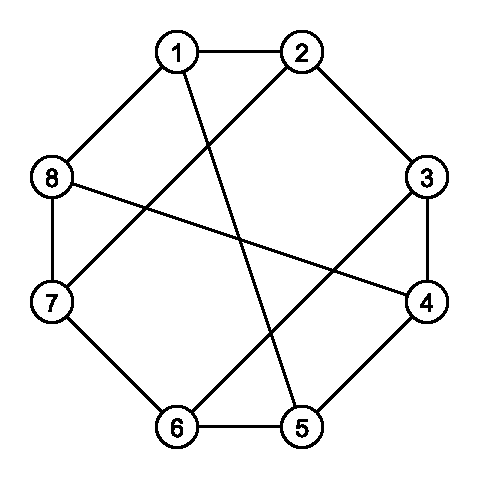
\includegraphics[width=0.2\linewidth]{example.pdf}
	\caption{Graph $G=(V,E)$. Let $H$ be the Hamiltonian cycle of $G$ that contains edges $(1,2),(2,3),(3,4),(4,5),(5,6),(6,7),(7,8),(1,8)$. Let $M= E\setminus H$: $M=\{(1,5),(2,7),(3,6),(4,8)\}$.}
	\label{example}
\end{figure}

Let $v^1$ be the following extreme point of $\EC(G)$: \begin{equation*}
v^1_{e} = \left\{ \begin{array}{ll}
1 & \mbox{if $e\in M$};\\
1/2 & \mbox{if $e\in H$}.
\end{array} \right. 
\end{equation*}
Define $z^1$ to be the following vector:
\begin{equation*}
z^1_{e} = \left\{ \begin{array}{ll}
7/5 & \mbox{if $e= (1,5)$};\\
1 & \mbox{if $e\in M\setminus \{(1,5)\}$};\\
2/5 & \mbox{if $e \in \{(1,8),((4,5))\}$};\\
3/5 & \mbox{if $e\in H\setminus\{(1,8),((4,5))\} $}.
\end{array} \right. 
\end{equation*}
It is easy to check that $z^1$ satisfies the requirement of Theorem \ref{gap} when setting $C=\frac{6}{5}$. In particular, we have $ z^1(\delta(U))\leq \frac{6}{5}v^1(\delta(U))$ for all $\emptyset\subset U \subset V$. Also, is it easy to decompose $z^1$ into a convex combination of integer point in of $\EC(G)$.

Now, we want to set the $\epsilon_i$ in the statement of Lemma \ref{epsilon} to be $2^{-k}$. By Lemma \ref{epsilon}
\begin{equation*}
x^1_{e} = \left\{ \begin{array}{ll}
\frac{2^k-7/6}{2^k-1} & \mbox{if $e= (1,5)$};\\
\frac{2^k-5/6}{2^k-1} & \mbox{if $e\in M\setminus \{(1,5)\}$};\\
\frac{2^k- 2/3}{2\cdot (2^k-1)} & \mbox{if $e \in \{(1,8),((4,5))\}$};\\
\frac{1}{2} & \mbox{if $e\in H\setminus\{(1,8),((4,5))\} $}.
\end{array} \right. 
\end{equation*}
is in $\EC(G)$ for sufficiently large $k$. The vectors defined below $v^2,\ldots,v^7$ are also extreme points of $\EC(G)$.

\begin{table}[h]
	\centering
	\begin{tabular}{ccccccccccccc}
		\toprule
		& (1,5) & (2,7)& (3,6)&(4,8)&(1,2)&(2,3)&(3,4)&(4,5)&(5,6)&(6,7)&(7,8)&(1,8)      \\ \midrule
			$v^2=$ & (0&1&2&1&0&1&1&2&0&0&1&2)  \\
			$v^3=$ & (0&2&2&1&0&0&0&1&1&1&1&2)\\
			$v^4=$ & (1&2&2&2&1&1&1&1&0&0&0&0)\\
			$v^5=$ & (0&2&1&1&1&1&0&1&1&0&0&1)\\
			$v^6=$ & (1&1&1&2&0&1&0&0&1&0&1&1)\\
			$v^7=$ & (1&1&1&2&1&0&1&1&0&1&0&0)\\
				 \bottomrule
	\end{tabular}
\end{table}
Moreover, we have 
\begin{equation*}
x^1 = (1-8\lambda)v^1+ \lambda v^2 + 2\lambda v^3+\lambda v^4+ \lambda v^5+ \lambda v^6 + 2\lambda v^7, \quad \lambda = \frac{1}{24\cdot (2^k-1)}
\end{equation*}
Now, this allows us to rewrite Inequality \ref{equation6} for this example.
\begin{equation*} 
\frac{6}{5}v^1 \geq \frac{3}{4} z^1 +\frac{1}{32}(\frac{6}{5}\cdot v^2) +\frac{1}{16}(\frac{6}{5}\cdot v^3) + \frac{1}{32}(\frac{6}{5}\cdot v^4)+\frac{1}{32}(\frac{6}{5}\cdot v^5) + \frac{1}{32}(\frac{6}{5}\cdot v^6)+ \frac{1}{16}(\frac{6}{5}\cdot v^7).  
\end{equation*}
\end{example}


\nocite{fj}\nocite{32gap}\nocite{TSPcompute}\nocite{abe}
\bibliographystyle{plain}
\bibliography{FDT}



\end{document}

